\chapter{Optimerings metoder} \label{kap:optimeringsmetoder}

Der er flere forskellige måder, at løse et lasso problem, hvis problemet er konveks. 
Vi introducerer to efficiente algoritmer for at løse lasso problemet, de er henholdsvis \textit{ LARS  (Least Angle Regression) algoritmen} og \textit{coordinate descent algoritmen}.

\section{LARS metode}
LARS algoritmen var først introduceret i \citep{efron}.  
Vi introducerer først den originale version af LARS algoritmen, hvor efter vi laver en simple modifikation af LARS algoritmen for at løse lasso. 

Ideen bag algoritmen er, at vi først sætter alle koefficienter lig nul, hvor vi herefter finder den , $x_{1j}$, som er mest korrelerede med respons variablen, $\textbf{y}$.  
Vi tager hernæst den størst mulige trin i retningen af vores prædiktor, hvor vi anvender en simple lineær regression af $\textbf{y}$ på $x_{1j}$. 
Vi får en residual vektor, som er ortogonal på $x_{j1}$ og bliver vores nye respons. 
Vi fortsætter indtil $x_{2j}$ er lige så korrelerede  med residualerne, som $x_{j1}$. 
LARS algoritmen anvender herefter den ensvinklet retning mellem $x_{1j}$ og $x_{2j}$, som den nye retning indtil den rammer den tredje variable, som er den mest korrelerede, hvorefter den nye retning er ensvinklet mellem de de tre variable $x_{1j}$, $x_{2j}$ og $x_{3j}$. Dette fortsættes. 

I hvert trin bliver der tilføjet en kovariat til vores model $\widehat{\boldsymbol{\mu}} = \textbf{X} \widehat{\boldsymbol{ \beta}}$, så efter $k$ iterationer er der k elementer i  $\widehat{\beta}_j$, som er forskellige fra nul.  

Figur \ref{fig:lars} illustrerer algoritmen, hvor $p = 2$ og $X = \del{\textbf{x}_1, \textbf{x}_2}$. 
Vi lader kovariaterne være standardiseret med middelværdi 0 og unit varians og lader respons have en middelværdi 0. Den nuværende korrelation er givet ved 
\begin{align*}
\textbf{c}\del{\boldsymbol{\widehat{\mu}}} = X^T\del{\textbf{y} - \widehat{\boldsymbol{\mu}}} = X^T \del{ \textbf{y}_2 - \boldsymbol{\widehat{\mu}}}.
\end{align*}
I dette tilfælde er den nuværende korrelation kun afhængige af projektionen $\textbf{y}_2 $, som er projektionen af $\textbf{y}$ i det lineære rum $L(X)$ udspændt af $ \textbf{x}_1 $og $\textbf{x}_2$. 
Algoritmen starter i $\widehat{\boldsymbol{\mu}}_0 = \textbf{0}$, hvor vi ser på figur \ref{fig:lars} at $ \textbf{y}_2 - \boldsymbol{\widehat{\mu}}_0$ og $\textbf{x}_1$ har den mindste vinkel i forhold til $ \textbf{y}_2 - \boldsymbol{\widehat{\mu}}_0$  og $\textbf{x}_2$, dvs at $\textbf{c}_1\del{\boldsymbol{\widehat{\mu}}_0} > \textbf{c}_2\del{\boldsymbol{\widehat{\mu}}_0}$. 
LARS algoritmen forstærker  $\boldsymbol{\widehat{\mu}}_0$ i retning af $\textbf{x}_1$ ved
%
 \begin{align*}
 \boldsymbol{\widehat{\mu}}_1 = \boldsymbol{\widehat{\mu}}_0 + \widehat{\gamma}_1 \textbf{x}_1.
 \end{align*}
 %
 Lad $\widehat{\gamma}$ være stepsize og bestemmes  således at $ \textbf{y}_2 - \boldsymbol{\widehat{\mu}}$ er lige korrelerede med $\textbf{x}_1$ og $\textbf{x}_2$, dvs det er når  $\textbf{y}_2 - \boldsymbol{\widehat{\mu}}_1$ deler vinkel i lige står dele mellem  $\textbf{x}_1$ og $\textbf{x}_2$, således at $\textbf{c}_1\del{\boldsymbol{\widehat{\mu}}_1} = \textbf{c}_2\del{\boldsymbol{\widehat{\mu}}_1}$.  
 
 Vi lader $\boldsymbol{\mu}_2$ være en enheds vektor liggende på bisektoren. Den næste LARS estimat er 
 %
 \begin{align*}
 \boldsymbol{\widehat{\mu}}_2 = \boldsymbol{\widehat{\mu}}_1+ \widehat{\gamma}_2 \boldsymbol{\widehat{\mu}}_2,
 \end{align*}
%
hvor $\widehat{\gamma}_2$ er valgt således at  $ \boldsymbol{\widehat{\mu}}_2 = \textbf{y}_2$ i tilfældet hvor $p = 2$. 
\begin{figure}
\centering
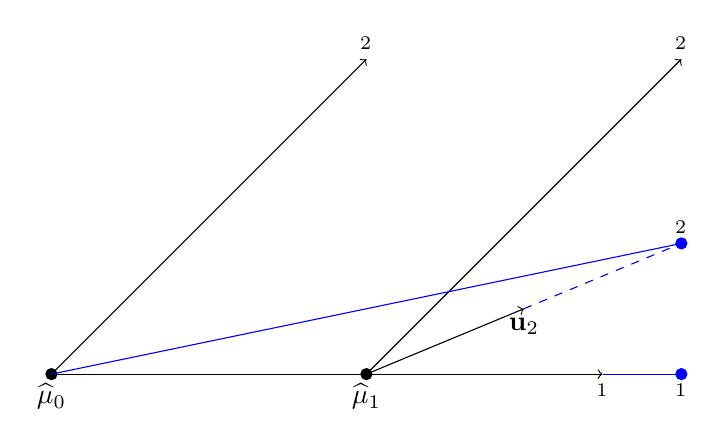
\begin{tikzpicture}
\draw [<-] (4,0) node [below] {$\x_1$}-- (-3,0);
\filldraw (1,0) circle (2pt) node [below] {$\widehat{\boldsymbol{\mu}}_1$};
\filldraw (-3,0)  circle (2pt) node [below]{$\widehat{\boldsymbol{\mu}}_0$};
\draw [<-] (5,4) node [above] {$\x_2$} --(1,0);
\draw [<-] (1,4) node [above] {$\x_2$} --(-3,0);

\draw [blue](5,1.66)  node [above, black] {$\y_2$} -- (-3,0);

\draw [->](1,0) -- (3, 0.83)  node [below] {$\mathbf{u}_2$} ;
\draw [dashed, blue] (3,0.83) -- (5,1.66) ; 


\filldraw [blue] (5,1.66) circle (2pt) ;
\draw [blue]  (5,0) node [below] {} -- (4,0);
\filldraw [blue] (5,0) circle (2pt) ;
\draw (5,0) node [black, below] {$\y_1$};
\end{tikzpicture} 
\caption{Figuren viser LARS algoritmen, i tilfældet hvor $p = 2$. Vi har to kovariater  $\textbf{x}_1$ og $\textbf{x}_2$, $\textbf{y}_2$ er projektionen af $\textbf{y}$ in i det lineære rum $L  \del{ \textbf{x}_1, \textbf{x}_2} $. }\label{fig:lars}
\end{figure}

Vi vil beskrive algoritmen mere generelt.
Vi antager at kovariaterne $ \textbf{x}_1,  \textbf{x}_2,  \dots,  \textbf{x}_p$ er lineært uafhængige og lader $\mathcal{A}$ være en delmængde af indekser $\{1, 2, \dots, p \}$. 
Vi definerer følgende mængder 
%
\begin{align*}
X_{\mathcal{A}} & = \del{\cdots s_j \textbf{x}_j \cdots}  \nonumber \\ 
N_{\mathcal{A}} & = X^T_{\mathcal{A}} X_{\mathcal{A}} \\ \
A_{\mathcal{A}} & = \del{ \textbf{1}^T_{\mathcal{A}} N_{\mathcal{A}} \textbf{1}_{\mathcal{A}} }^{- 1/2} , \nonumber 
\end{align*}
%
hvor  $s_j = \pm 1$ og $\textbf{1}_{\mathcal{A}} $ er en vektor bestående af 1-taller, som har samme længde som $\abs{\mathcal{A}}$. 
Lad 
%
\begin{align*}
\textbf{u}_{\mathcal{A}} = X_{\mathcal{A}} \omega_{\mathcal{A}}, 
\end{align*}
%
kaldes den ensvinklet vektor og hvor $ \omega_{\mathcal{A}} = A_{\mathcal{A}} G^{-1}_{\mathcal{A}}  \textbf{1}^T_{\mathcal{A}}$. 

Der gælder følgende 
%
 \begin{align*}
 X^T_{\mathcal{A}} \textbf{u}_{\mathcal{A}} = A_{\mathcal{A}}  \textbf{1}_{\mathcal{A}}   \quad  \text{og} \quad \norm{ \textbf{u}_{\mathcal{A}}}^2 = 1.
\end{align*}  
%
Derudover lad $\widehat{c}$ være en vektor af nuværende korrelationer, lad $\widehat{C}$ være den maksimale nuværende absolut korrelation, og lad $s_j$ være fortegnet af $\widehat{c}$: 
%
\begin{align*}
 \widehat{\textbf{c}} & = X^T \del{ \textbf{y}- \widehat{\boldsymbol{\mu}}}, \\
 \widehat{C} & = \max_j \cbr{\abs{\widehat{c}_j}}, \\
 s_j &  = \text{sign} \cbr{\widehat{c}_j}, \quad \text{for } j \in \mathcal{A},
\end{align*}
%
hvor $\widehat{\boldsymbol{\mu}} = X \widehat{\beta}$ er det nuværende LARS estimat. Vi definerer den aktive mængde $\mathcal{A}$, som en mængde af indekser som tilhører de kovariater, som har den maksimale nuværende absolut korrelation med de nuværende remanens (residuum?).  Dvs 
\begin{align*}
\mathcal{A} = \cbr{j : \abs{\widehat{c}_j} = \widehat{C}} = \cbr{j : \widehat{\beta}_j \neq 0},
\end{align*}

\begin{alg} [LARS algoritme]
\begin{enumerate}
%
\item Standardiserer prædiktorerne til at have en middelværdi 0 og $\norm{\textbf{x}_j}_2^2$ for alle $j$.
Vi starter med $\widehat{\boldsymbol{\mu}}_0 = 0$, $\widehat{\boldsymbol{c}} = X^T \textbf{y}$ og $\widehat{\boldsymbol\beta}_0 = \del{0, \dots, 0}^T$
%
\item Find prædiktoren $\textbf{x}_j$ med den højest værdi af  $ \abs{\widehat{c}_j}$ og definer den aktive mængde $\mathcal{A} = \cbr{j}$. 
%
\item Gentag følgende indtil alle prædiktoreren fra den komplementærmængde $\mathcal{A}^C$ er indeholdt i det aktive mængde
%
\begin{itemize}
%
\item Udregn  $\widehat{\textbf{c}}$, $ \widehat{C} $, $ X_{\mathcal{A}}$,$ A_{\mathcal{A}}$,  $\textbf{u}_{\mathcal{A}}$ ud fra overstående formler og det indre produkt vektor
%
\begin{align*}
\textbf{a} = X^T \textbf{u}_{\mathcal{A}} = \del{a_1, \dots, a_p}^T
\end{align*}
%
\item Opdaterer $\widehat{\boldsymbol{\mu}}_{\mathcal{A}}$ ved
\begin{align}
\widehat{\boldsymbol{\mu}}_{\mathcal{A}} = \widehat{\boldsymbol{\mu}}_{\mathcal{A}} + \widehat\gamma \textbf{u}_{\mathcal{A}} \label{eq:u}
\end{align}
%
hvor
\begin{align}
\widehat\gamma = \underset{j \in \mathcal{A}^C}{\min^+} \cbr{ \frac{\widehat{C}- \widehat{c}_j}{A_\mathcal{A} - a_j} \frac{\widehat{C} + \widehat{c}_j}{A_\mathcal{A} + a_j}}, \label{eq:j_indeks}
\end{align}
hvor $\min^+$ betyder, at minimum kun er taget af positive komponenter for hvert valg af $j$. 
\item Mængden $\mathcal{A} = \mathcal{A} \cup \widehat{j}$, hvor $\widehat{j}$ er den maksimale indeks i \eqref{eq:j_indeks}. 
\end{itemize}
\end{enumerate}
\end{alg}
Overstående viser hvordan algoritmen bliver brugt. Men for lasso skal der bruges en lille modifikation. 
Vi lader $\widehat{\boldsymbol\beta} = \del{\widehat{\beta}_1, \dots, \widehat{\beta}_p }^T$ være en lasso løsning til $\widehat{\boldsymbol{\mu}} = X \widehat{\boldsymbol\beta}$. Der gælder at fortegnet af enhver estimerede koefficient $\beta_j$ må have samme fortegn som den nuværende korrelation $\widehat{c}_j = \textbf{x}_j \del{\textbf{y} - \widehat{\mu}}$, 
\begin{align*}
\text{sign} \del{\widehat{\beta}_j} = \text{sign} \del{\widehat{c}_j} = s_j
\end{align*}
...... (bevis) 

For at tage den her modifikation i betragtning tilføjer vi følgende i tredje trin. 
\begin{itemize}
\item Definerer p-vektoren $\widehat{\textbf{d}} = s_j \omega_{\mathcal{A}_j}$ for $j \in \mathcal{A}$ og er ellers nul. Hvor $ \omega_{\mathcal{A}_j}$ betegner j'te elementet af vektoren $\omega_{\mathcal{A}}$. 
\item For $j \in \mathcal{A}$ opdaterer vi 
\begin{align*}
\widehat{\beta}_j \del{\gamma} = \widehat{\beta}_j + \gamma \widehat{d}_j 
\end{align*}
\item Vi lader 
\begin{align*}
\gamma_j = - \frac{\widehat{\beta}_j}{\widehat{f}_j} \quad \text{og} \quad \tilde\gamma = \underset{y_j > 0}{\min} \cbr{\gamma_j}. 
\end{align*}
\item Hvis $\gamma = \tilde{\gamma}$, så træk det$ \tilde{j}$'te elemeent fra udregning af den næste ensvinklet retning, dvs 
\begin{align*}
\widehat{\boldsymbol\mu}_{\mathcal{A}_+} = \widehat{\boldsymbol\mu}_\mathcal{A} + \tilde{\gamma} \textbf{u}_\mathcal{A} \quad \text{og} \quad \mathcal{A_+} = \mathcal{A}- \cbr{\tilde{j}}
\end{align*}
udregnes i stedet for \eqref{eq:u}.
\end{itemize}

Flere beskrivelser af algoritmen kan findes i \citep{efron}. 
LARS har følgende fordele.
En af dem er, at den giver en ranking af prædiktorer når der bliver tilføjet andre prædiktorer, som ikke er tilfældet med hard treshold. 
En anden fordel er at algoritmen undgår streng korrelerede prædiktorer, hvis en af de korrelerede prædiktorer allerede er inkluderet, siden at den nye residual vil have lav korrelation med variabler, som er streng korrelerede variabler, som allerede er inkluderet. 
Derudover er LARS algoritmen ikke er 'greedy', som forward regression, fordi den udnytter en god retning til dens maksimum . 
LARS algortimen har også samme beregnings omkostninger, som en velkendt OLS \citep{hui_hastie}. 

\section{Coordinate Descent}
For at løse optimeringsproblemer kan Coordinate Descent anvendes. 
Coordinate Descent er en første ordens iterative algoritme, hvilket betyder der kun bruges gradienten af funktionen, som information. 
Hvis koordinat $k$ er valgt i iteration $t$, så får vi følgende opdaterings linje
\begin{align*}
\beta_k^{t+1} =\underset{ \beta_k}{\arg \min}  f\del{ \beta_1^t, \beta_2^t, \dots, \beta_{k-1}^t, \beta_k, \beta_{k+1}^t, \dots, \beta_p^t  },
\end{align*}
hvor $\beta_j^{t+1} = \beta_j^t$ for $j \neq k$. 
Der er to basale modeller for coordinate algoritmer i forhold til den måde de opdaterer parametrene. Den første er cyclic coordinate og den anden kaldes greedy coordinate. 
Cyclic opdaterer en parameter i hvert loop og den greedy opdaterer parameteren, som giver den største ændring i funktionen. 

Coordinate algoritmer er generelt rigtig anvendt, når man skal estimerer parameter af en funktion, som ikke er differentiable. Sådan en funktion kunne se følgende ud
\begin{align*}
f(\beta_1, \dots, \beta_p) = g(\beta_1, \dots, \beta_p) + \sum_{j = 1}^p h_j \del{\beta_j},
\end{align*}
hvor $g: \R^p \rightarrow \R $ er differentialble og konveks, og hvor den univariate funktion $h_j : \R \rightarrow \R$ er konveks (ikke nødvendigvis differentialble). Udfra Tseng .... kan det vises at en hver konveks funktion, som $f$, konvergerer coordinate descent til det globale minimum. 
?? bevis
 


